\chapter{Effective Field Theory}
\label{chap:EFT}

\section{Low Energy EFT}
\label{sec:LEFT}

\begin{figure}[tbh!]
 \begin{center}
 \begin{tabular}{cc}
 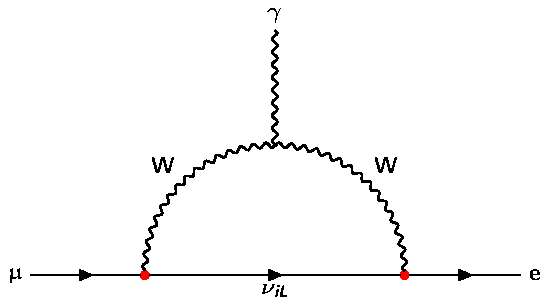
\includegraphics[width=0.45\textwidth]{figures/Part1/EFT/mutoe}&
 \includegraphics[width=0.45\textwidth]{figures/Part1/EFT/fermimutoe}\\
 \end{tabular}
 \caption{Representative Feynman diagrams for $\upmu^{-}\rightarrow\textsf{e}^{-}\nu_{\upmu}\bar{\nu}_{\textsf{e}}$ decay. The \ac{SM} description of this phenomenon with a massive weak mediator is illustrated on the left. At low energy, the heavy weak boson is approximated to be point-like in Fermi's theory of weak interactions, which is illustrated on the right. The effective coupling between four fermions, indicated with a red dot, can be used to describe the same phenomenon.}
 \label{fig:FermiEFT}
 \end{center}
\end{figure}

\begin{figure}[tbh!]
 \begin{center}
 \begin{tabular}{cc}
 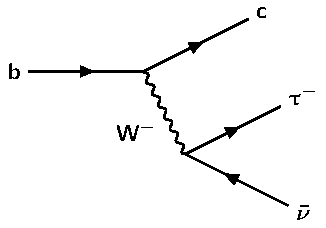
\includegraphics[width=0.45\textwidth]{figures/Part1/BSM/SMbtoc}&
 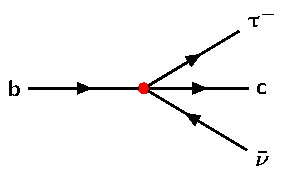
\includegraphics[width=0.5\textwidth]{figures/Part1/EFT/LEFT}
 \end{tabular}
 \caption{Representative Feynman diagram for $\rightarrow$c transtion in the \ac{SM} (left). This process might also be enhanced by new physics with a much higher energy scale. The potential contributions from new physics can therefore be described by an effective coupling between four fermions, which is illustrated on the right.}
 \label{fig:LEFT}
 \end{center}
\end{figure}

\section{Standard Model EFT}
\label{sec:SMEFT}